\documentclass[dvipdfmx]{ujarticle}
\usepackage[dvipdfmx]{graphicx}
\usepackage{here}
%% 高さの設定
\setlength{\textheight}{\paperheight}   % ひとまず紙面を本文領域に
\setlength{\topmargin}{-5.4mm}      % 上の余白を20mm(=1inch-5.4mm)に
\addtolength{\topmargin}{-\headheight}  % 
\addtolength{\topmargin}{-\headsep}     % ヘッダの分だけ本文領域を移動させる
\addtolength{\textheight}{-50mm}    % 下の余白も20mmに
%% 幅の設定
\setlength{\textwidth}{\paperwidth}     % ひとまず紙面を本文領域に
\setlength{\oddsidemargin}{-5.4mm}  % 左の余白を20mm(=1inch-5.4mm)に
\setlength{\evensidemargin}{-5.4mm} % 
\addtolength{\textwidth}{-40mm}     % 右の余白も20mmに
\pagestyle{empty}   %ページ番号なし

\newcommand{\g}[1]{\boldsymbol{#1}}
\newcommand{\lw}[1]{\smash{\lower2.0ex\hbox{#1}}}
\renewcommand{\baselinestretch}{1.0}

\makeatletter
\def\mojiparline#1{
    \newcounter{mpl}
    \setcounter{mpl}{#1}
    \@tempdima=\linewidth
    \advance\@tempdima by-\value{mpl}zw
    \addtocounter{mpl}{-1}
    \divide\@tempdima by \value{mpl}
    \advance\kanjiskip by\@tempdima
    \advance\parindent by\@tempdima
}
\def\linesparpage#1{
    \baselineskip=\textheight
    \divide\baselineskip by #1
}

\title{単一QD-SOAを用いた全光XOR-AND回路}
\author{4616072 畑洋樹}

\begin{document}
\mojiparline{43}

\begin{center}
  % title
  {\Large \textbf{単一QD-SOAを用いた全光半加算器}}
\end{center}
\begin{flushright}
畑 洋樹 (八嶋 弘幸 教授, \  柴田 凌 助教)
\end{flushright}
\vspace{-3zw} 

\section{はじめに}
  近年のインターネット通信端末の増加と普及により,光通信による通信の高速化と大容量化が必要不可欠となっている.
  現在の光通信では,信号処理を行う際に一度光信号から電気信号へと変換するため,通信速度の最大値が電気信号の処理速度に依存してしまうという課題がある.
  従って電気信号への変換処理が必要ない全光信号処理技術を構成する全光論理回路の研究が進められている.
  また,従来研究として実装されている全光論理回路の多くは光がデバイスに入射した際に発生する非線形光学効果を利用している.
  その中でも量子ドット半導体光増幅器(Quantum-Dot Semiconductor Optical Amplifiers: QD-SOA)を用いた全光論理回路が提案されている.
  QD-SOAは量子ドット構造の活性層を持つ光増幅器のことであり,電子を量子ドット内に閉じ込めることで従来の光増幅器よりも大きな利得を得ることができる. \\
  従来研究として提案されている全光XOR回路ではマッハツェエンダー干渉計(Mach-Zehnder Interferometer:MZI)を用いた回路が提案されている.
  しかし,MZIを用いた全光回路は同一特性のQD-SOAを2つ使用しなければならず,同一特性のQD-SOAを製造することは非常に困難という問題がある.
  上記の問題点を踏まえ、特定の波長の光を切り出すデバイスであるOptical Filter(OF)の波長を任意に変更することで出力としてXOR回路としてだけでなくAND回路としても使用できる.

\section{従来研究}
  \subsection{非線形光学効果}
    弱い光によって生じる光の直進,屈折,回折といった様々な光学効果はすべて線形光学効果と呼ばれる.
    ここでいう線形とは光に対する物質の応答が光電場によって比例しているということである.
    これは光の電界によって発生する分極によるものであるが,光の強度が大きくなると分極が光の強度に比例しなくなり非線形性が見られることがある.
    これが光の非線形光学効果の発生原理である.
    \subsubsection{相互位相変調(XPM)}
    光カー効果により物質の屈折率が変化することで物質を進む光の位相が変化する.
    この現象を利用することでクロック光の強度を変化させることにより入射光の位相を制御させることができる.
    \subsubsection{相互利得変調(XGM)}
    QD-SOAの光の増幅利得は有限であり入力光強度が大きくなるとそれ以上光を増幅できない.
      この特性を利用することでクロック光の強度を変化させることにより入射光の利得を制御させることができる.

\section{提案する単一QD-SOAを用いた全光半加算器}
  \begin{figure}[H]
    \begin{center}
      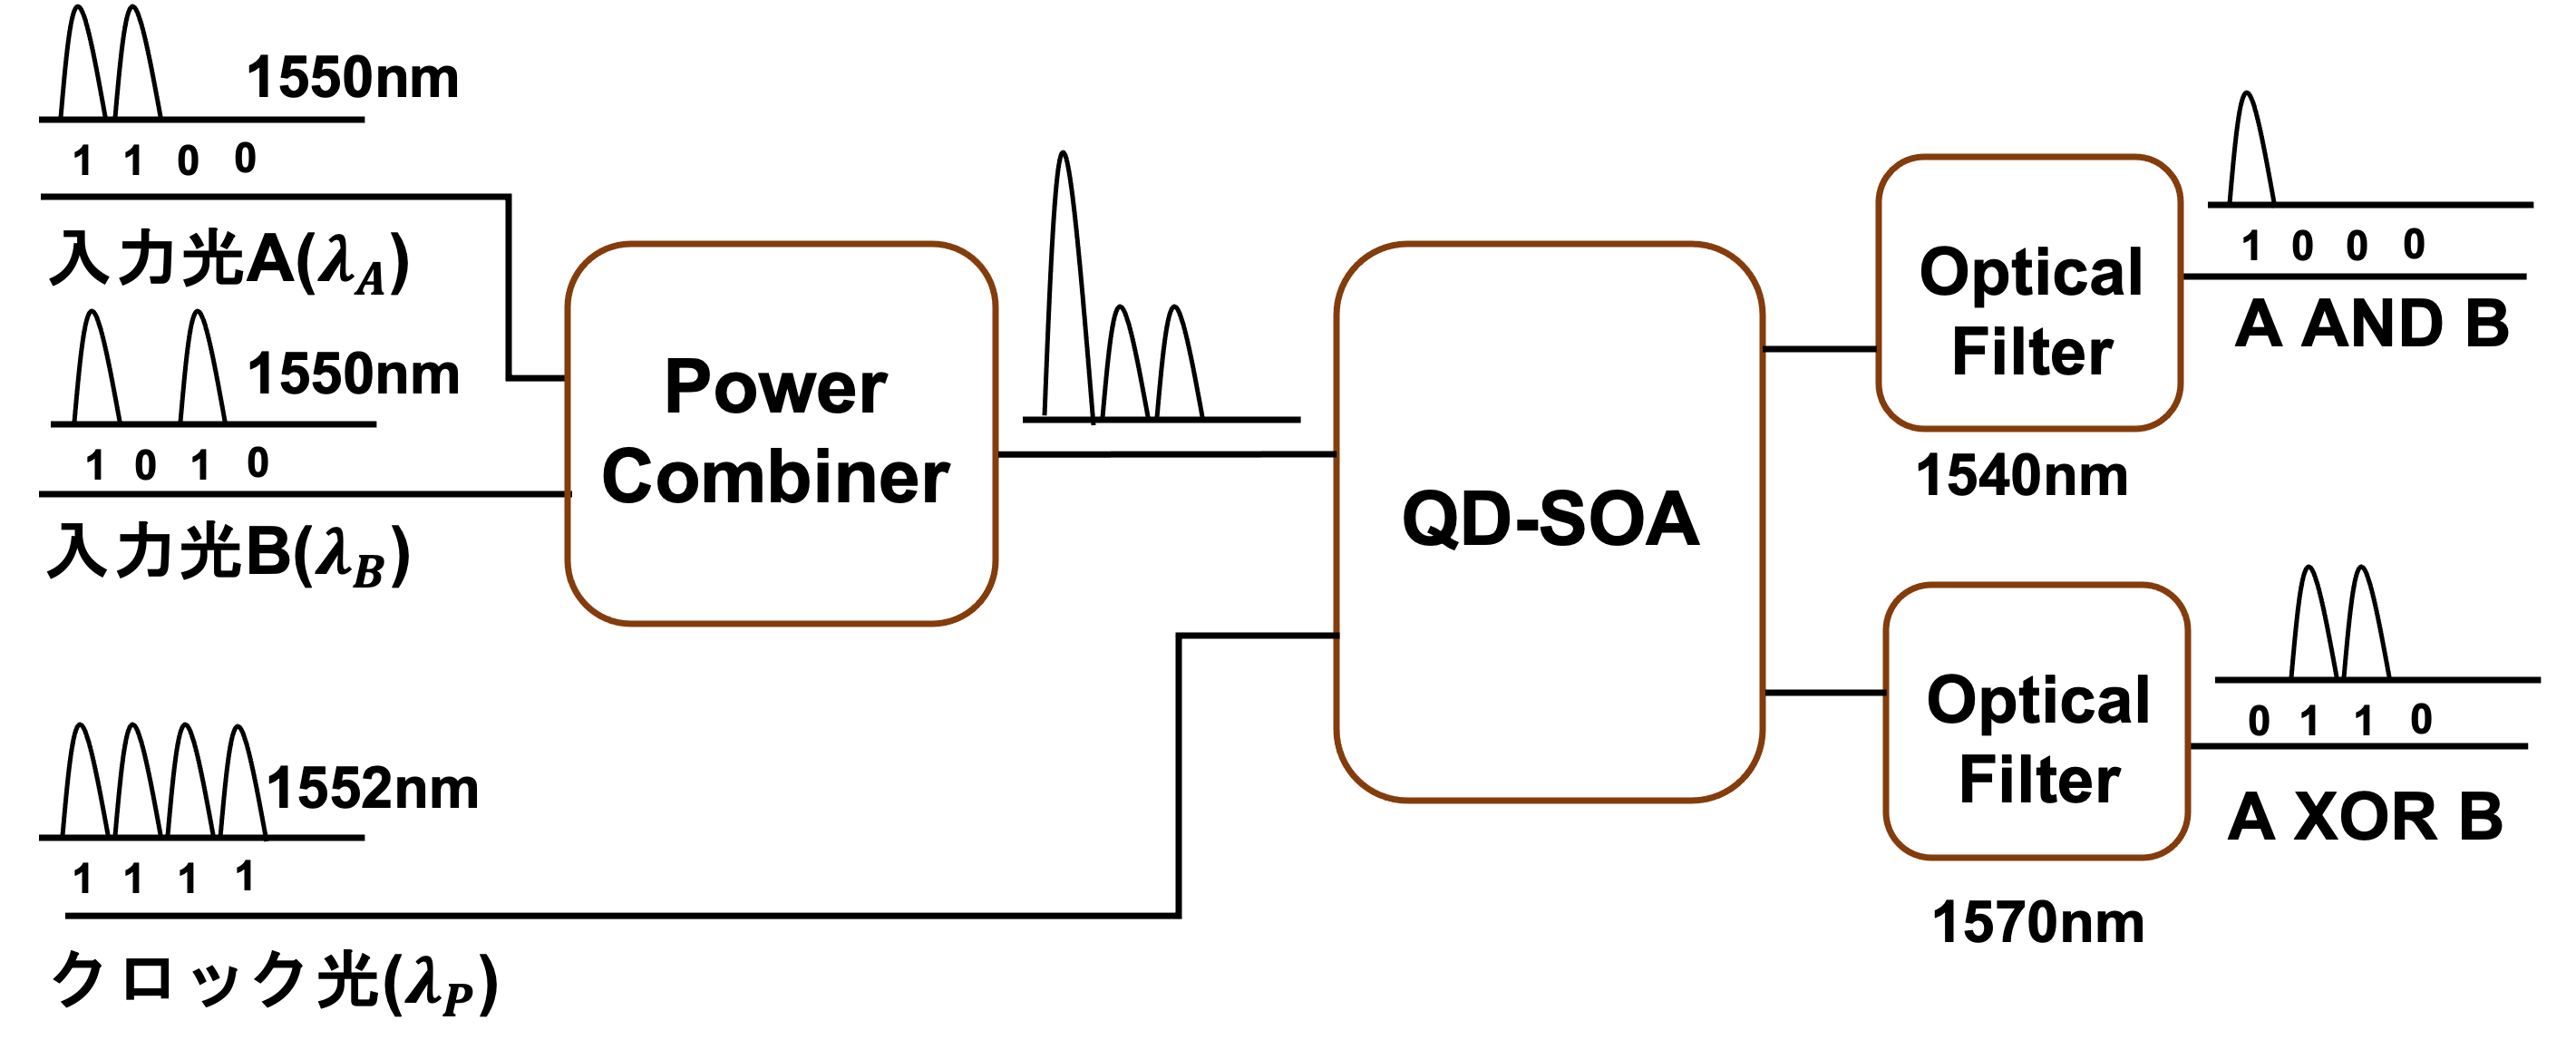
\includegraphics[width=15cm]{images/kairo.png}
      \caption{提案する全光半加算器の構成}
    \end{center}
  \end{figure}
  提案する全光回路ではまず, 入力光A,Bを複数の光を合波するデバイスであるPowerCombiner(PC)に入射させる.
  その後合波された光とクロック光をQD-SOAに入力させることにより,光スペクトルが変化する.
  最後に特定の波長の光を切り出すデバイスであるOptical Filter(OF)を用いて基本論理回路として必要な波長のみを取り出し最終的な出力光とする.
  \subsection{光フィルタの波長選択}
    入力光の値によるQD-SOAからの出力スペクトラムを下記に示す. \\
    光フィルタを用いて実践で囲った波長を分離するとXOR演算として機能し, 破線で囲った波長を分離するとAND演算として機能する.
    \begin{figure}[H]
      \begin{tabular}{cc}
        \begin{minipage}[t]{0.45\hsize}
          \centering
          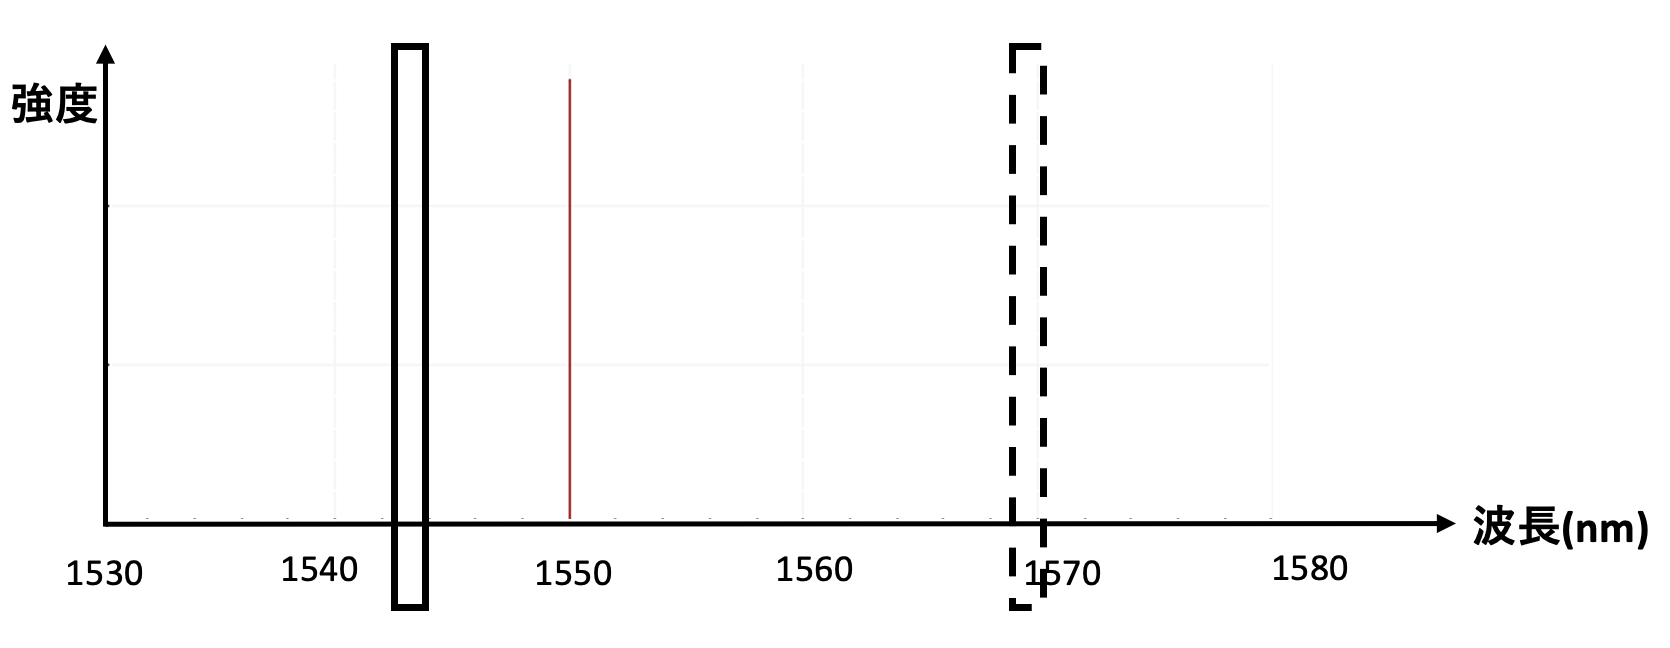
\includegraphics[width=7cm]{images/00_spectrum.png}
          \caption{入力光A=0, 入力光B=0の場合のスペクトラム}
        \end{minipage} &
        \begin{minipage}[t]{0.45\hsize}
          \centering
          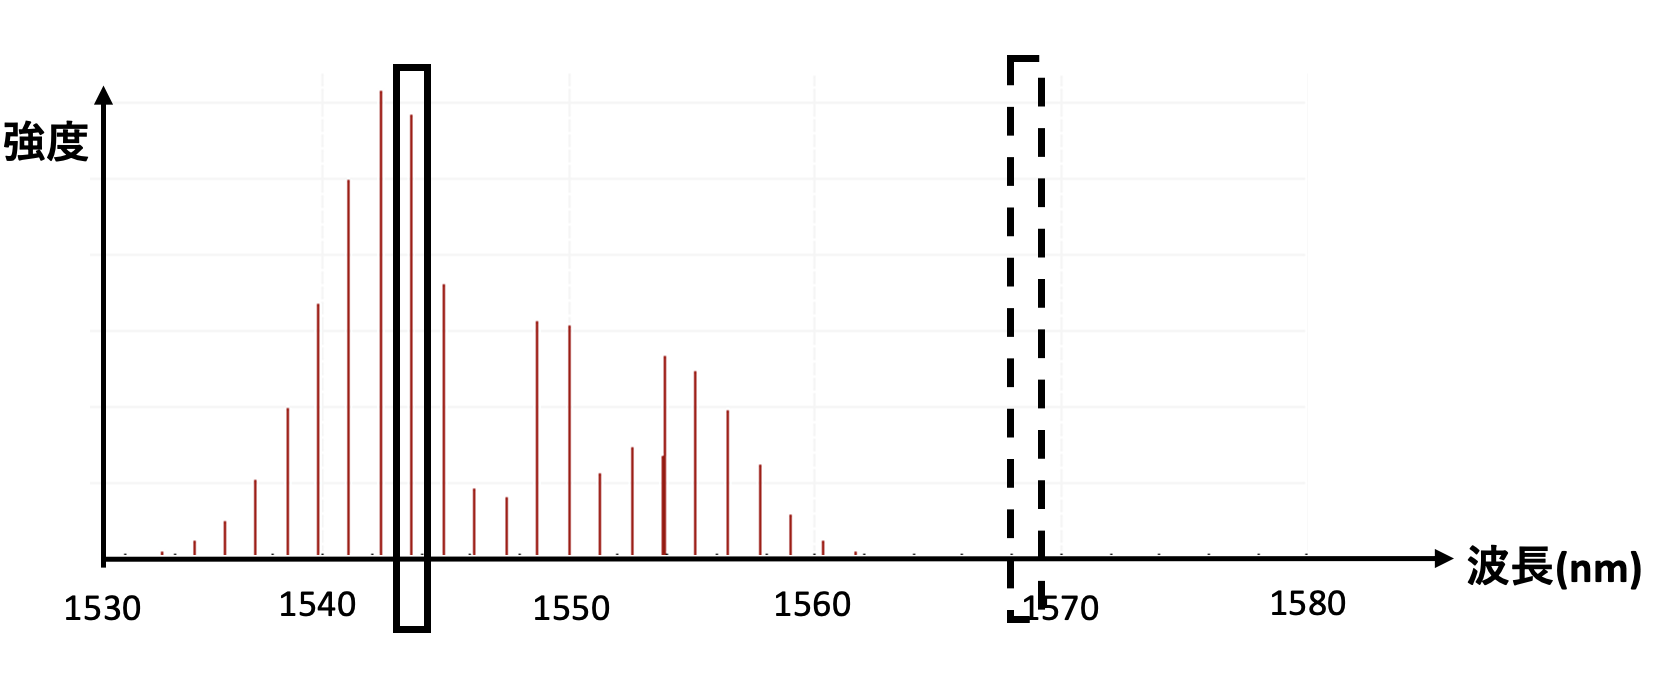
\includegraphics[width=7cm]{images/01_spectrum.png}
          \caption{入力光A=1, 入力光B=0の場合のスペクトラム}
        \end{minipage}
        \\
        \begin{minipage}[t]{0.45\hsize}
          \centering
          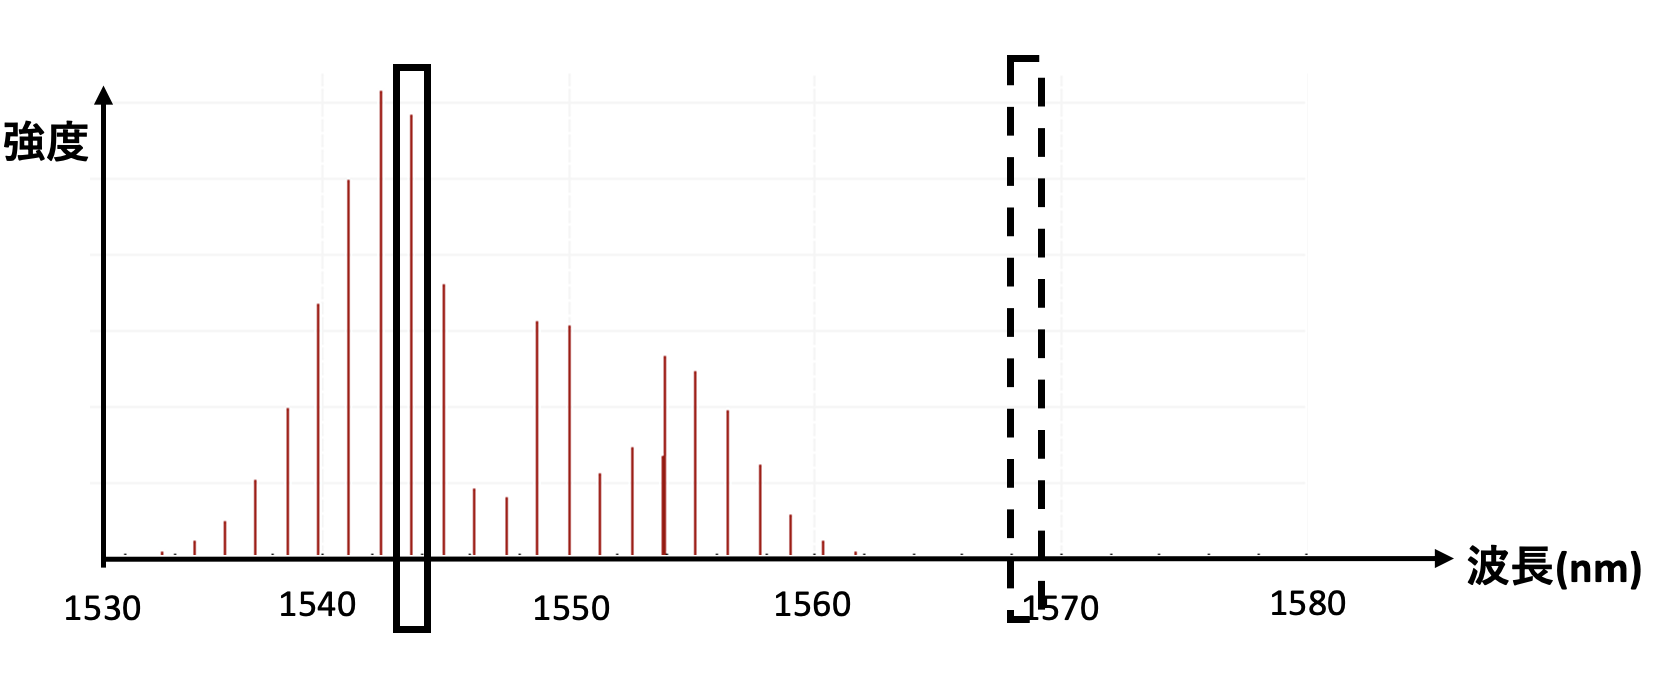
\includegraphics[width=7cm]{images/01_spectrum.png}
          \caption{入力光A=0, 入力光B=1の場合のスペクトラム}
        \end{minipage} &
        \begin{minipage}[t]{0.45\hsize}
          \centering
          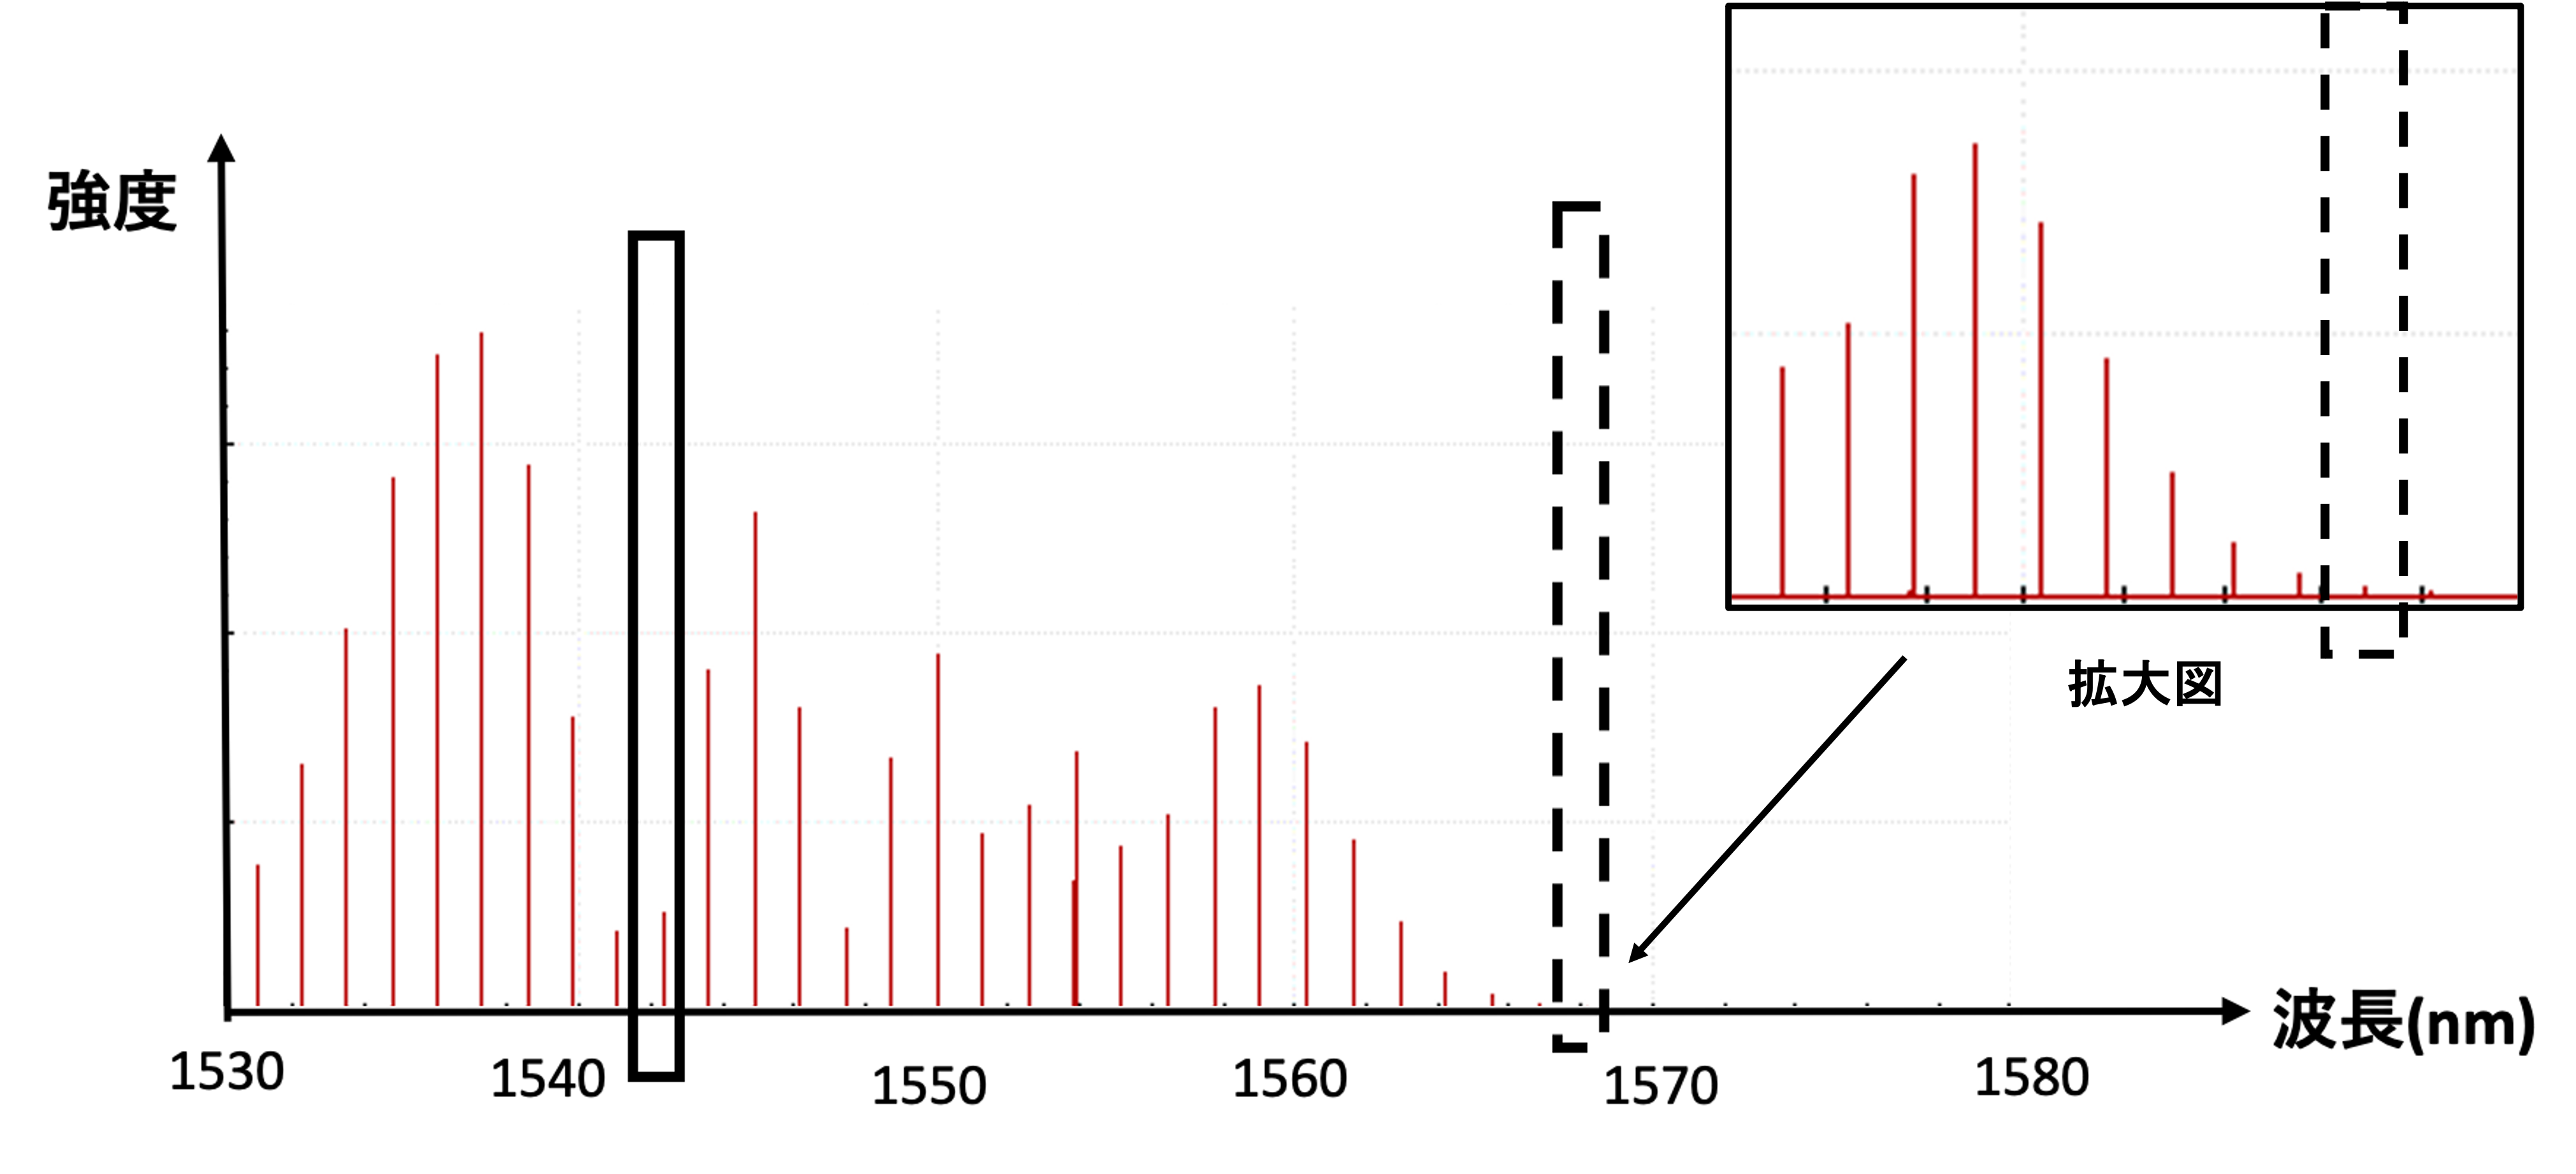
\includegraphics[width=7cm]{images/11_spectrum.png}
          \caption{入力光A=1, 入力光B=1の場合のスペクトラム}
        \end{minipage}
      \end{tabular}
    \end{figure}
    \begin{itemize}
      \item 入力光が互いに0の場合 \\
      QD-SOA内で非線形光学効果が発生せずクロック光が大きく増幅される.
      \item 入力光のどちらかのみが1の場合 \\
      QD-SOA内で非線形光学効果であるXGMによって入力光に利得が奪われるためクロック光があまり増幅されない.
      さらにXPMによってスペクトルが広がる.
      \item 入力光が互いに1の場合 \\
      XGMによってクロックはほとんど増幅されない.
      さらにXPMによってどちらかが1の場合よりもスペクトルが大きく広がる
    \end{itemize}

\section{シミュレーション}
  \subsection{条件及び評価指標}
    本研究では OptiSystem16.1.0, MATLAB 2019a を用いてシミュレーションを行った.
    QD-SOAは光の伝搬方程式, キャリアのレート方程式及び伝達行列法(Transfer Matrix Method:TMM)を用いてシミュレーションを行った.ビットレートは160Gbpsとした.
    光の伝搬方程式はQD-SOA内の光電界に関する式であり,キャリアのレート方程式はQD-SOA内の時間変化によるキャリアの変化を表す式である.
    また,伝達行列法はQD-SOAを光の伝搬方向に対して細かく分割しキャリア密度, 光子密度, 利得を繰り返し求めることで結果的に出力される光電界を求める手法である.
    今回シミュレーションで使用するパラメータは表1[1]に示したものを用いた.\\
     シミュレーションでは入力光強度と各演算に対応する光フィルタの指定波長を変化させ、それぞれの条件に対する消光比が最も高くなるようなパラメータ探索を行う.
    なお,各演算に対応する光フィルタの指定波長はスペクトラムの広がりから指定する.
    \begin{table}[H]
      \caption{シミュレーションで用いるパラメータ}
      \centering
        \begin{tabular}{ccc}
          \hline
          パラメータ名 & 値 & 単位 \\
          \hline
          QD-SOAの長さ & $ 3.0 \times 10^{-3} $ & $m$\\
          QD-SOAの厚さ & $ 0.25 \times 10^{-6} $ & $m$\\
          QD-SOAの幅 & $ 3.0 \times 10^{-6} $ & $m$\\
          量子ドット密度 & $ 5.0 \times 10^{14} $ & $m^{-2}$\\
          キャリア寿命(WL→ES) & $ 3.0 \times 10^{-12} $ & $s$ \\
          キャリア寿命(ES→WL) & $ 1.0 \times 10^{-9} $ & $s$\\
          キャリア寿命(WL→系外) & $ 2.0 \times 10^{-9} $ & $s$\\
          キャリア寿命(ES→GS) & $ 0.16 \times 10^{-12} $ & $s$\\
          キャリア寿命(GS→ES) & $ 1.2 \times 1o^{-12} $ & $s$\\
          キャリア寿命(GS→系外) & $ 0.4 \times 10^{-9} $ & $s$\\
          注入電流 & $5.0 \times 10^{-2}  $ & $A$\\
          最大利得 & $12.0 $ & $cm^{-1}$\\
          損失係数 & $2.0$ & $cm^{-1}$\\
          \hline
        \end{tabular}
    \end{table}

  \subsection{評価指標}
    評価指標としてアイダイアグラム(eye diagram)および消光比(Extinction Ratio: ER)を用いる.
    アイダイアグラムとは信号光を1ビット幅間隔で分割し,重ね合わせて描画したグラフのことであり,
    消光比は ${P^1}_{min}$を “1” として出力された光の中で最も強度が弱いときの光強度の値,
    ${P^0}_{min}$を “0” として出力された光の中で最も強度が強い時の光強度の値としたときに
    $ER[dB] = 10 \log{10}{\frac{{P^1}_{min}}{{P^0}_{max}}}$ で算出される指標である.
    この値が大きいほど出力光が “0” , “1” の区別がつきやすい優れた波形であることを示す.

  \subsection{シミュレーション結果}
    AND演算およびXOR演算を行った場合のシミュレーション結果をアイダイアグラムの形で描画すると図6,7のように表せる.
    AND演算における消光比は14.88dB, XOR演算における消光比は11.03dBが得られた.
    \begin{figure}[H]
      \begin{tabular}{cc}
        \begin{minipage}[t]{0.45\hsize}
          \centering
          \includegraphics[width=7cm]{images/AND_RESULT.png}
          \caption{AND回路の結果}
        \end{minipage} &
        \begin{minipage}[t]{0.45\hsize}
          \centering
          \includegraphics[width=7cm]{images/XOR_RESULT.png}
          \caption{XOR回路の結果}
        \end{minipage}
      \end{tabular}
    \end{figure}

\section{まとめ}
  単一QD-SOAを用いた全光AND/XOR論理回路を提案した.
  シミュレーション結果より論理回路の動作を確認でき, 評価指標から出力波形の品質は良好と見られる.
  今後の課題としてより現実状態に近い性能評価を行うため,QD-SOA内で生じるASE雑音の考慮が挙げられる.

\begin{thebibliography} {99}
  \bibitem{1} H.Sun, Q.Wang, H.Dong and N.K.Dutta, “XOR performance of a quantum dot semiconductor optical amplifier based MachZehnder interferometer”, Department of Physics, University of Connecticut, Storrs, CT 06269, 2005.
  \bibitem{2} E.Dimitriadou K.E.Zoiros, “All-Optical XOR Gate Using Single Quantum-Dot SOA and Optical Filter”, Journal of lightwave Technology, vol.31, NO.23, Dec. 2013.
  \bibitem{3} 古松 幸輔, “All-optical NOR gate using a single quantum-dot SOA-assisted an optical filter,“ Opt, Quant. Electron., 東京理科大学平成 29 年度修士論文.
  \bibitem{4} 北山研一著 光通信工学, オーム社, 2012.
\end{thebibliography}

\end{document}
